%%%%%%%%%%%%%%%%%%%%%%%%%%% asme2e.tex %%%%%%%%%%%%%%%%%%%%%%%%%%%%%%%
% Template for producing TSFP-format articles using LaTeX
% Based on the asme2e template (http://iel.ucdavis.edu/code/ASME/)
% Modified: 11 February 2013 for TSFP8 by R. Manceau
% Modified: 05 May 2014 for TSFP9&10 by K. Chauhan
% In case of problem: kapil.chauhan@sydney.edu.au
%%%%%%%%%%%%%%%%%%%%%%%%%%%%%%%%%%%%%%%%%%%%%%%%%%%%%%%%%%%%%%%%%%%%%%

%%%%%%%%%%%%%%%%%%%%%%%%%%%%%%%%%%%%%%%%%%%%%%
% To generate a pdf, compile either with pdflatex
% or with latex and
% dvips tsfp_template -Ppdf -t a4 -o
% followed by
% ps2pdf tsfp_template.ps
% (avoid using dvipdf that does not preserve the page layout on some systems)
%%%%%%%%%%%%%%%%%%%%%%%%%%%%%%%%%%%%%%%%%%%%%%

%%% use twocolumn and 10pt options with the tsfp format
\documentclass[twocolumn,10pt]{tsfp}
\usepackage{graphicx}% Include figure files
\usepackage{dcolumn}% Align table columns on decimal point
\usepackage{bm}% bold math
\usepackage{MnSymbol}
\usepackage{gensymb}
\usepackage{stackengine}
\usepackage{color}
\usepackage[authoryear,round]{natbib}
\usepackage{color}

\title{REYNOLDS DECOMPOSITION OF TURBULENCE CONTAINING SUPER-COHERENT STATES}

%%%% In case you need to slightly adapt the horizontal spacing between authors (for more than 3 authors) uncomment the following command
%%%% and if necessary modify the factor
%\renewcommand{\expauthors}{1.1}

%%% first author
\author{R. J. Adrian, P. J. Sakievich, Y. T. Peet
    \affiliation{
	Mechanical and Aerospace Engineering\\
	School of Matter Transport and Energy, \\
	 Arizona State University\\
	501 E. Tyler Mall, Tempe, AZ 85287\\
    email: rjadrian@asu.edu
    }	
}

%%% second author
%%% remove the following entry for single author papers
%%% add more entries for additional authors
%\author{Philip J. Sakievich
%          \affiliation{
%	Mechanical and Aerospace Engineering\\
%	School of Matter Transport and Energy, \\
%	 Arizona State University\\
%	501 E. Tyler Mall, Tempe, AZ 85287\\
%    email: psakievi@asu.edu
%    }	
%}
%
%\author{Yulia T. Peet
%          \affiliation{
%	Mechanical and Aerospace Engineering\\
%	School of Matter Transport and Energy, \\
%	 Arizona State University\\
%	501 E. Tyler Mall, Tempe, AZ 85287\\
%    email: ypeet@asu.edu
%    }	
%}
\begin{document}

\maketitle   %Print title matter

% Set the font to 9pt.
\fontsize{9}{11}\selectfont

%%%%%%%%%%%%%%%%%%%%%%%%%%%%%%%%%%%%%%%%%%%%%%%%%%%%%%%%%%%%%%%%%%%%%%
\section*{ABSTRACT}
A vexing problem occurs in certain flows when long, but finite, time-average estimates of the mean flow fail to exhibit the symmetry properties imposed by boundary conditions and physics. The mean field becomes suspect, making it difficult, or even incorrect to apply Reynolds decomposition. The problem occurs when the flow exhibits ?super-coherent? states, i.e. states of flow having coherence times much longer than the averaging times used in typical turbulence experiments. Turbulent Rayleigh-B\'{e}nard convection (RBC) is one such flow, and it will be used here as an example to illustrate and explain this phenomenon. The study focuses on a turbulent RBC experiment~\citep{fernandes2001spatial} in a 6.3:1 (diameter: depth) aspect-ratio vertical cylinder that supplemented time averaging with true ensemble averaging to achieve almost zero mean flow. To obtain a three-dimensional time-varying picture of the mechanisms at work, the experiment is simulated by direct numerical simulation of the Boussinesq equations~\citep{sakievich2016large}. Three types of super-coherent states, associated with the symmetries of the flow, are found to bias the mean flow, unless steps are taken to sample each state with equal probability.  
%%%%%%%%%%%%%%%%%%%%%%%%%%%%%%%%%%%%%%%%%%%%%%%%%%%%%%%%%%%%%%%%%%%%%%
%%%%%%%%%%%%%%%%%%%%%%%%%%%%%%%%%%%%%%%%%%%%%%%%%%%%%%%%%%%%%%%%%%%%%%
\section*{INTRODUCTION}
Reynolds decomposition is fundamental in the analysis of turbulence, and measurement of the mean flow must be accurate to within a small fraction of the turbulent fluctuation intensity to properly define the turbulent fluctuating field. The rules for averaging the results of turbulent flow experiments, physical or numerical, are quite simple: infinite averages over time are unbiased if the flow is statistically stationary and ergodic; infinite averages over space are unbiased if the flow is statistically homogeneous in the averaging direction(s) and ergodic; and finite averages converge to the infinite averages with small random error if they are performed over many thousand integral scales (in time or space). Lastly, convergence should be checked by repeated experiments.

  These rules suffice in most situations, if the averaging domains are large enough to achieve converged statistics, but not always. In certain flows they do not guarantee unbiased results because, even if convergence is suggested by smoothness of the average, it may be much slower may be much slower than expected, leading to physically incorrect results. Very slow convergence occurs when coherent structures of the flow, usually those of large scale, persist over times much longer than scale analysis or the integral time scale would suggest. We call structures having this property ?super-coherent?. The failure of the integral time scale to disclose super-coherence lays in the fact that it is composed of the time scales of motions of all sizes, such that the scale-scale, sort-time motions skew the correlation function to small times, thereby obscuring the long-time motions. 
 
A more insidious problem with time averaging occurs when the flow locks into 'states' that do not possess all of the symmetry that the infinite time average must have. These seem to result from state-space bifurcations into basins of attraction that trap the dynamics for very long (or perhaps infinite), times only occasionally (or perhaps never) allowing natural transitions from one basin to another. In these cases, averages over long but finite times may sample only one of the states, or sample one state over a much longer time than another, creating a bias. It is necessary to either take much longer time averages, many times not an option, or to stimulate the transitions. The latter can be accomplished by stopping the experiment and starting a new one, so as to achieve identical, independent experiments, yielding a finite ensemble of equi-probable experiments. This approach holds true to the definition of an ensemble average, and so long as each state is realized with equal frequency, it is shown to improve convergence to the true infinite time average considerably \citep{fernandes2001spatial}. 

    Two new methods are introduced to reduce bias to one state or another in a finite time experiment. One involves sensing the times spent in the different states, and the other defines an efficient way to stop and restart the identical experiments so as to achieve independent realizations whose initial conditions occupy the various basins of attraction with the correct frequency of occurrence.

\section*{TURBULENT RAYLEIGH-B\'{E}NARD CONVECTION}
     The ideal canonical form of RBC occurs in a horizontal layer of constant property fluid bounded by two infinitely wide horizontal plates, the warm bottom plate being heated uniformly and steadily, and the cool top plate being cooled in a similar manner to achieve either constant temperatures or constant mean heat flux.   
%
%RBC occurs when fluid between horizontal plates is heated from below and cooled from above.  
The unstable temperature stratification generates buoyancy forces within the fluid layer which then drive the flow. The Rayleigh number $Ra=\beta g \Delta T h^3/\alpha \nu$, (where $\beta$ is the coefficient of thermal expansion, $g$ is the gravitational constant, $\Delta T$ is the temperature difference between the two heated plates, $h$ is the plates' vertical separation, $\alpha$ is the thermal diffusivity and $\nu$ is the kinematic viscosity), is the primary dimensionless parameter and the Prandtl number $Pr=\nu/\alpha$ is often of less importance. A horizontal length scale ($L$) is also very important for determining the structure of the flow. The ratio of these two length scales is the aspect-ratio ($\Gamma=L/h$).

    Linear instability of this system occurs at $Ra=1708$, and it has the form of parallel, steady, two-dimensional roll-cells. With increasing Rayleigh number a sequence of more complicated finite amplitude laminar instabilities and transitions occurs \citep{busse1971instabilities,busse1974oscillatory,busse1978non}, ending with steady, laminar hexagonal cells at about $Ra=50,000$. Above $Ra= 10^5$ the flow becomes chaotic, and around $Ra=10^6-10^7$ it is usually considered to be turbulent. Studies of the turbulent state \citep{chu1973turbulent,garon1973velocity,willis1970oscillatory,fitzjarrald1976experimental} were generally performed in square or rectangular test sections whose aspect ratios ranging from xx.x to xx.x. Despite having fairly wide aspect?ratios, the experiments capable of sensing the flow velocity found non-zero mean flows, contrary to the zero-value expected for infinite aspect-ratio. As noted above this puzzling result made application of Reynolds decomposition problematic. A similar phenomenon also appeared in unsteady non-penetrative convection, a very close relative of RBC in which the cool upper plate is replaced by an insulating plate \citep{adrian1986turbulent}. including side-walls and insufficient aspect-ratio that might favor flow in one direction more than another. But the careful experiments of \cite{krishnamurti1981large} iin an annular test section also possessed mean flows around the annulus, despite the absence of side-walls. showing conclusively that non-zero mean flow in RBC derives from mechanics of the flow rather than experimental imperfections

\section*{LOW ASPECT-RATIO CONVECTION}

Since the pioneering work of \cite{castaing1989scaling} on very high Rayleigh Rayleigh number turbulent convection in unit aspect-ratio cubes and cylinders found the Nusselt number proportional to $Ra^{0.278}$ rather than the accepted value of $Ra^{1/3}$ most research has focused on very high Rayleigh numbers, necessitating low aspect-ratio test sections (see the review by \cite{ahlers2009heat}) . 

It is commonly observed that mean flow is prominent in unit aspect-ratio cubes and cylinders \citep{zocchi1990coherent, bodenschatz2000recent,ahlers2009heat}). 
Originally called the 'wind of turbulence', the mean flow is part of a large-scale circulation that sweeps across the upper and lower plates, Fig. 1 creating a boundary layer that is of considerable interest regarding heat transfer.

Over the last two decades there has been a strong focus in the RBC community on understanding the scaling of the Nusselt number $(Nu)$ with respect to $Ra$ and $Pr$.  
As the years have progressed ever larger $Ra$ have been reached in experimental and numerical studies with the goals of defining the scaling behavior and reaching the 'ultimate' state for turbulent convection that was first proposed by \cite{kraichnan1962turbulent}.  
Many different scaling laws for characterizing the heat transfer scaling in RBC systems \citep{ahlers2009heat}, but the most seminal and enduring work over the last 20 years is the theory proposed by \cite{grossmann2000scaling}.   
Grossmann and Lohse initial publication for a unifying theory to predict the scaling of the Reynolds number $(Re)$ and Nusselt number $(Nu)$ in turbulent RBC for any given $Pr$ and $Ra$ occurred in 2000 and has been improved by several additional publications~\citep{grossmann2001thermal,grossmann2002prandtl,grossmann2003geometry,grossmann2004fluctuations,stevens2013unifying}.  
This theory relies on three main assumptions for the flow field: statistical stationarity, a single dominant velocity scale represented by a mean wind, and characteristic boundary layer thicknesses for respective kinematic and thermal fields. 
  
The majority of numerical and experimental studies have been performed in unit $\Gamma$ boxes and cylinders.  The 'wind of turbulence' concept is often used to describe the flow structure in these small $\Gamma$ domains.  
The 'wind of turbulence' is characterized by a single roll-cell, or large-scale circulation (LSC), which spans the height and width of the cell, see figure~\ref{fig:1ar}.  This roll-cell creates boundary layers along the side walls and thermally active top and bottom plates which are well described by the Prandtl-Blasius profiles according to \cite{grossmann2000scaling}.  
While the theory has proven remarkably robust in predicting the scaling of $Nu$, the underlying assumptions are not guaranteed to hold at larger $\Gamma$ where the large-scale structure of the flow departs from the concept of a single LSC.

\begin{figure}
\centering
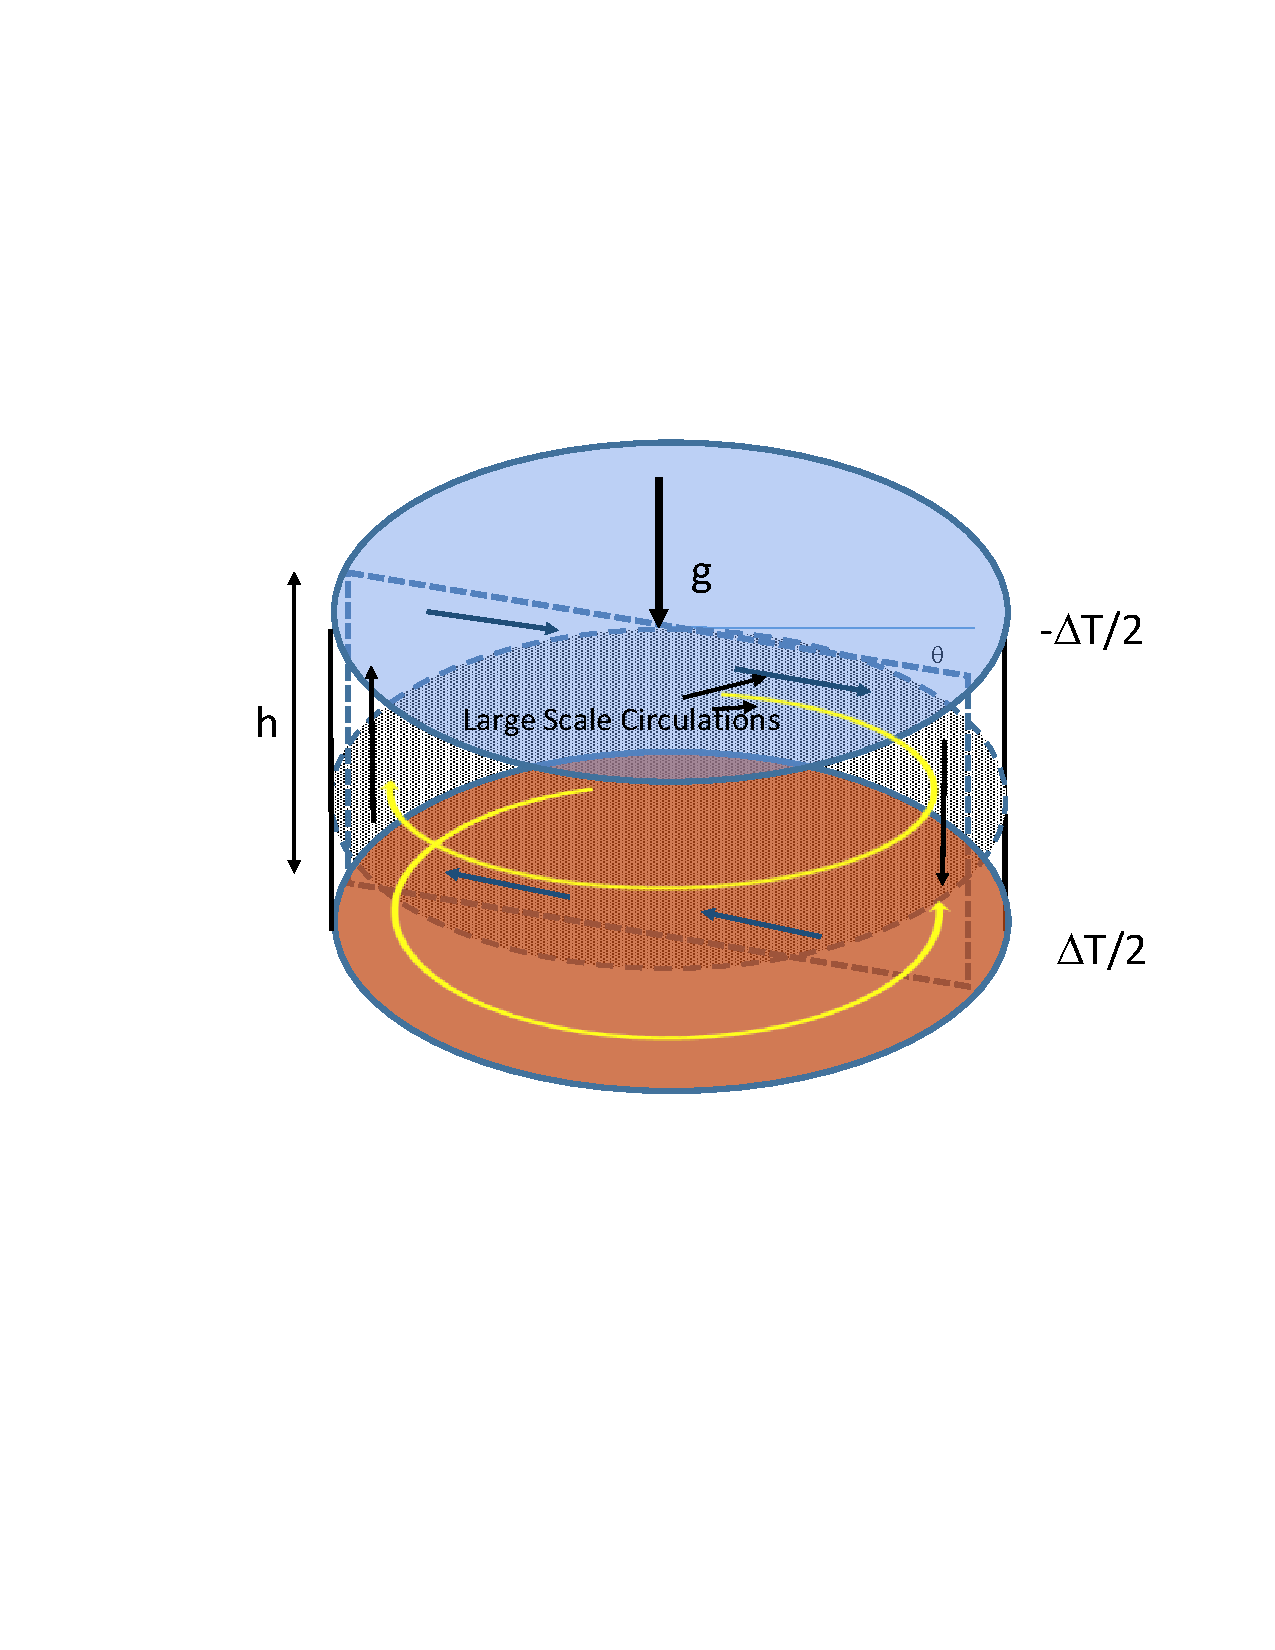
\includegraphics[trim=4cm 9cm 2cm 6cm, clip, width=7cm]{Ar1Sym}
\caption{Conceptual diagram of the wind of turbulence in a $\Gamma=1$ cell. The dotted plane illustrates the one of the infinite possibilities for the azimuthal orientation of the LSC. The yellow vectors indicate the directions for azimuthal drift.}
\label{fig:1ar}
\end{figure}

%For example, at a high enough $Ra$ the boundary layers within the system are expected to depart from the laminar, Prandtl-Blasuis description and move into a fully turbulent state (Ahlers \textit{et al.}, 2009).  
%Recent work at low $Pr$ by \cite{schumacher2016transitional} clearly shows patches of where the boundary layers are transitioning to fully developed turbulent profiles.  
%Extrapolation exercises align the work of \cite{schumacher2016transitional} experimental data from 'Uboot of G\:{o}ttingen' as outlined by \cite{ahlers2017ultimate}.  

For example, \cite{dupuits2007breakdown} clearly showed that the 'wind of turbulence' breaks down as $\Gamma$ increases by performing experiments in air over a wide range of $\Gamma=1-11$ and $Ra=10^8-10^11$.
This has been further corroborated by numerical studies of \cite{bailon2010aspect} ($Ra=10^7-10^9$, $\Gamma=0.5-11.0$)  and \cite{sakievich2016large} ($Ra=10^8$, $\Gamma=6.3$) that reveal complex multi-dimensional patterns for roll-cells in moderate $\Gamma$ containers with sidewalls.  
In a recent conference \cite{stevens2016superstructures} presented a numerical study that outlined the spatial extent needed to support true horizontal homogeneity in a periodic domain at $Ra=10^8$ and $Pr=1$.  
\cite{stevens2016superstructures} found that $\Gamma=32$ is required to support the full structure of the flow field, and that measured $Nu$ departs from the Grossmann-Lohse theory until $\Gamma>4$.  
These variations from the standard picture of $\Gamma=1$ RBC show that the physics of thermal convection is not fully described by the unit $\Gamma$ case, and that there is a clear value in returning to large$\Gamma$ studies that were prevalent several decades ago.

Very slowly evolving coherent motions have been observed in experimental studies and numerical simulations of wide aspect-ratio, turbulent Rayleigh-B\'{e}nard convection.  The time scales on which they evolve make it extremely difficult to achieve statistically-converged results during the finite run times of numerical simulations. In this paper, we present a novel procedure of manipulating the turbulent flow states and performing statistical averaging in a way that mitigates these problems and yields the flow statistics that are close to the results of experiments which, in turn, approach the infinite-time average.

Most theories of turbulence assume the flow is statistically stationary so that averages over infinite times converge to the ensemble average of an infinite number of random realizations. This makes the infinite-time average calculable in principle. In experiments and numerical simulations the infinite-time average is unreachable, and time averages over finite times often fail to converge well. Supplemental spatial averages over regions of homogeneous statistics or supplemental ensemble averages over additional realizations are often invoked to improve convergence of the finite-time average. 

\section*{SUPER-COHERENCE AND STATES OF TURBULENT RBC IN AN ASPECT-RATIO 6.3:1 CYLINDER}

\subsection*{FERNANDES EXPERIMENT}
At first blush one is tempted to attribute LSC?s to low aspect ratio, but as mentioned earlier, mean flow patterns have been observed in wider aspect-ratios, as well. The experiment by \cite{fernandes2001spatial} employed a $914mm \times  914mm$ convection with a cylindrical domain of diameter $760mm$ and height $120mm$ defined within by a thin, circular acetate wall. The aspect ratio was 6.3:1. With the intent of making the side-wall of the cylinder more passive thermally, convection occurred outside the cylinder as well as inside. 


\subsection*{PRESENT SIMULATION}
\begin{figure*}
\begin{center}
\topinset{\bfseries(a)}{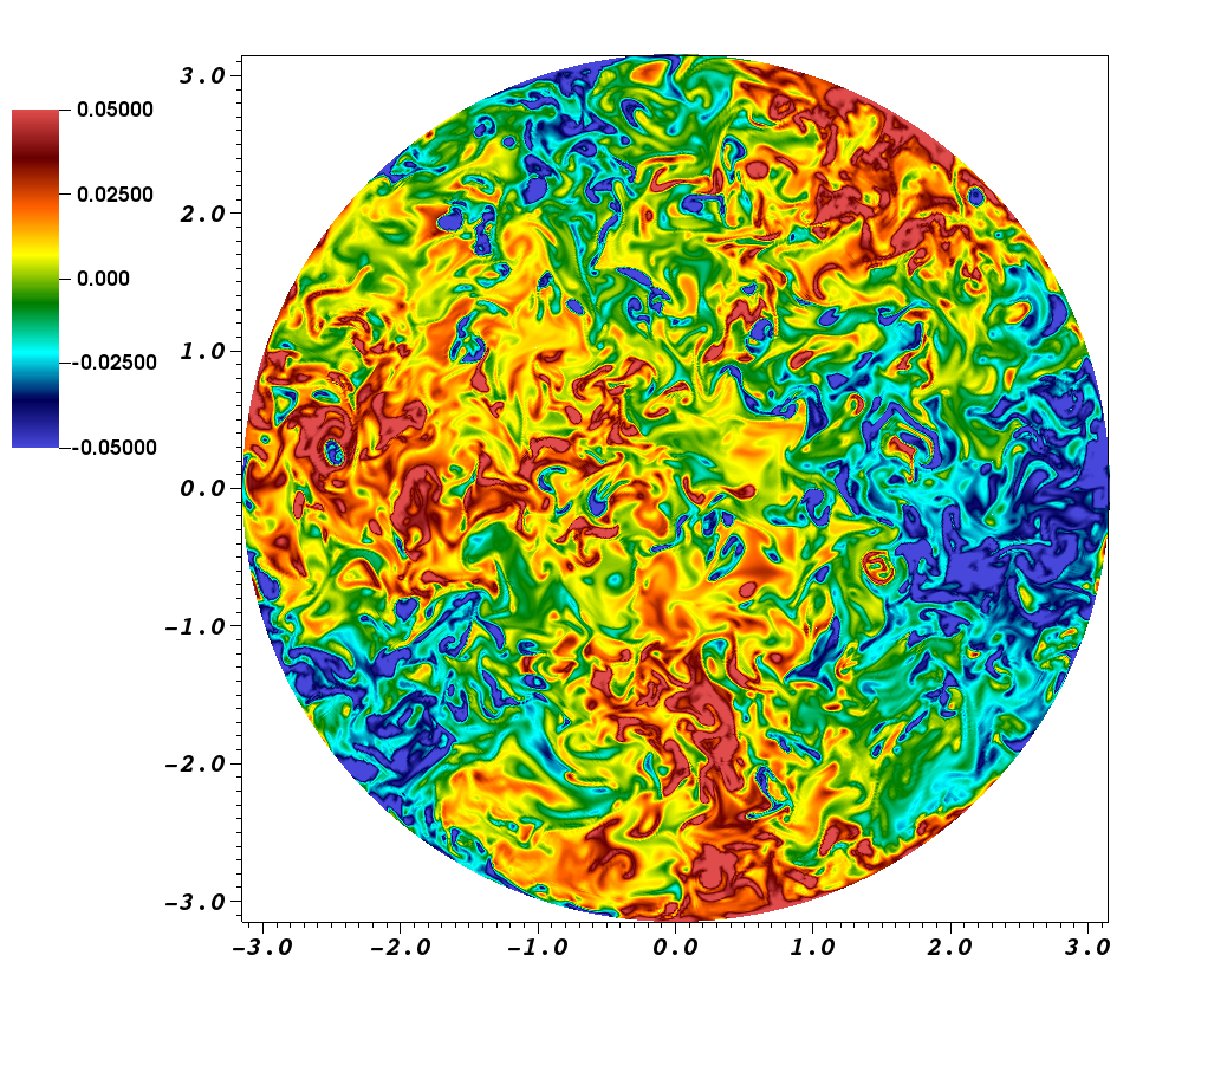
\includegraphics[trim=0cm 2cm 1cm 0cm,clip,width=0.23\textwidth]{TSFP_Filter_Width0000}}{0cm}{-0.1\textwidth}
\topinset{\bfseries(b)}{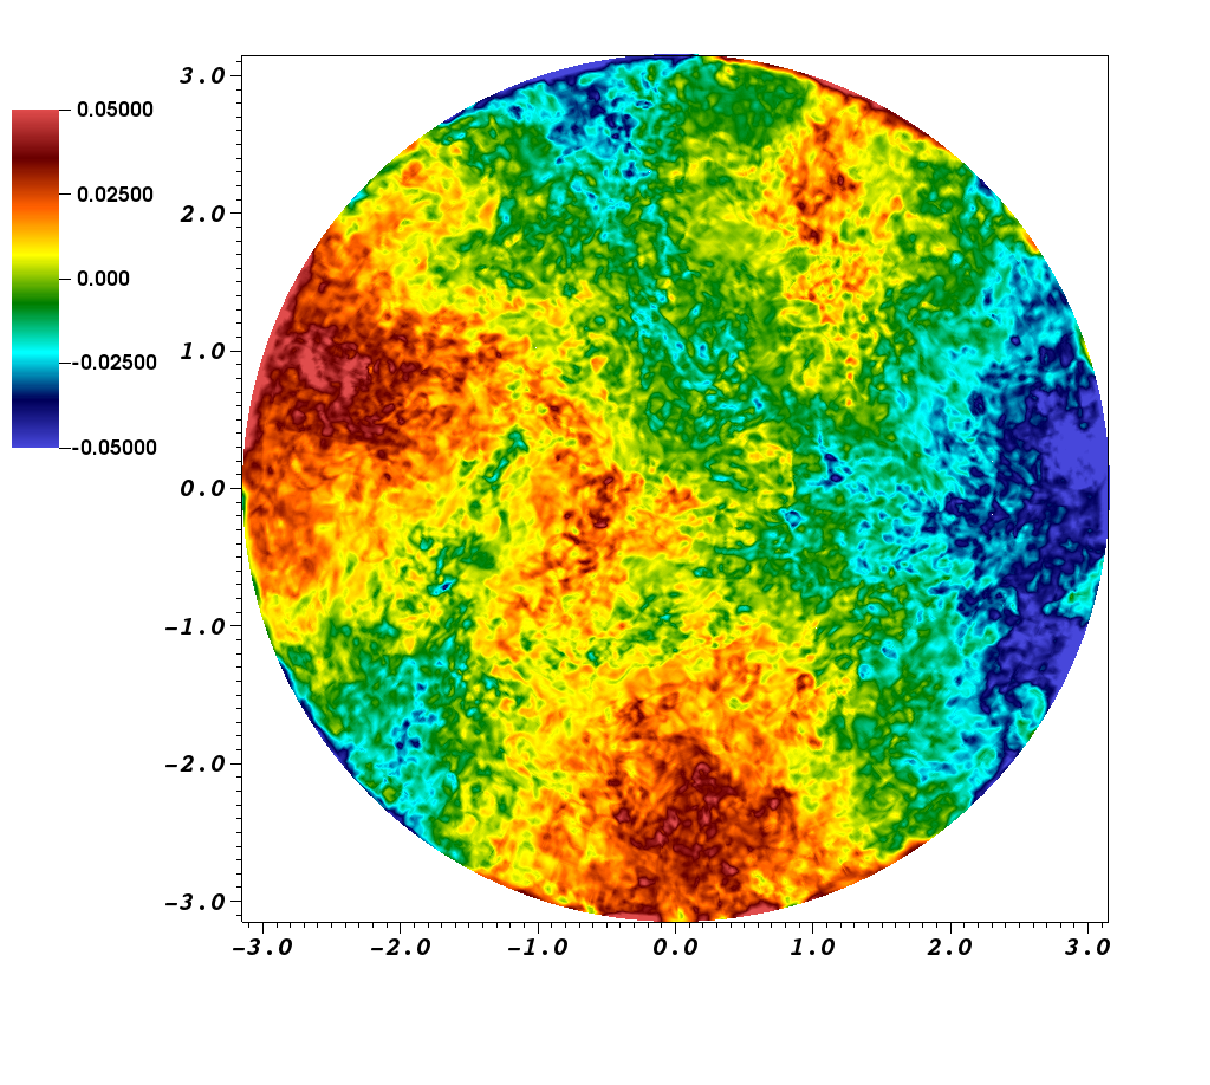
\includegraphics[trim=0cm 2cm 1cm 0cm,clip,width=0.23\textwidth]{TSFP_Filter_Width0001}}{0cm}{-0.1\textwidth}
\topinset{\bfseries(c)}{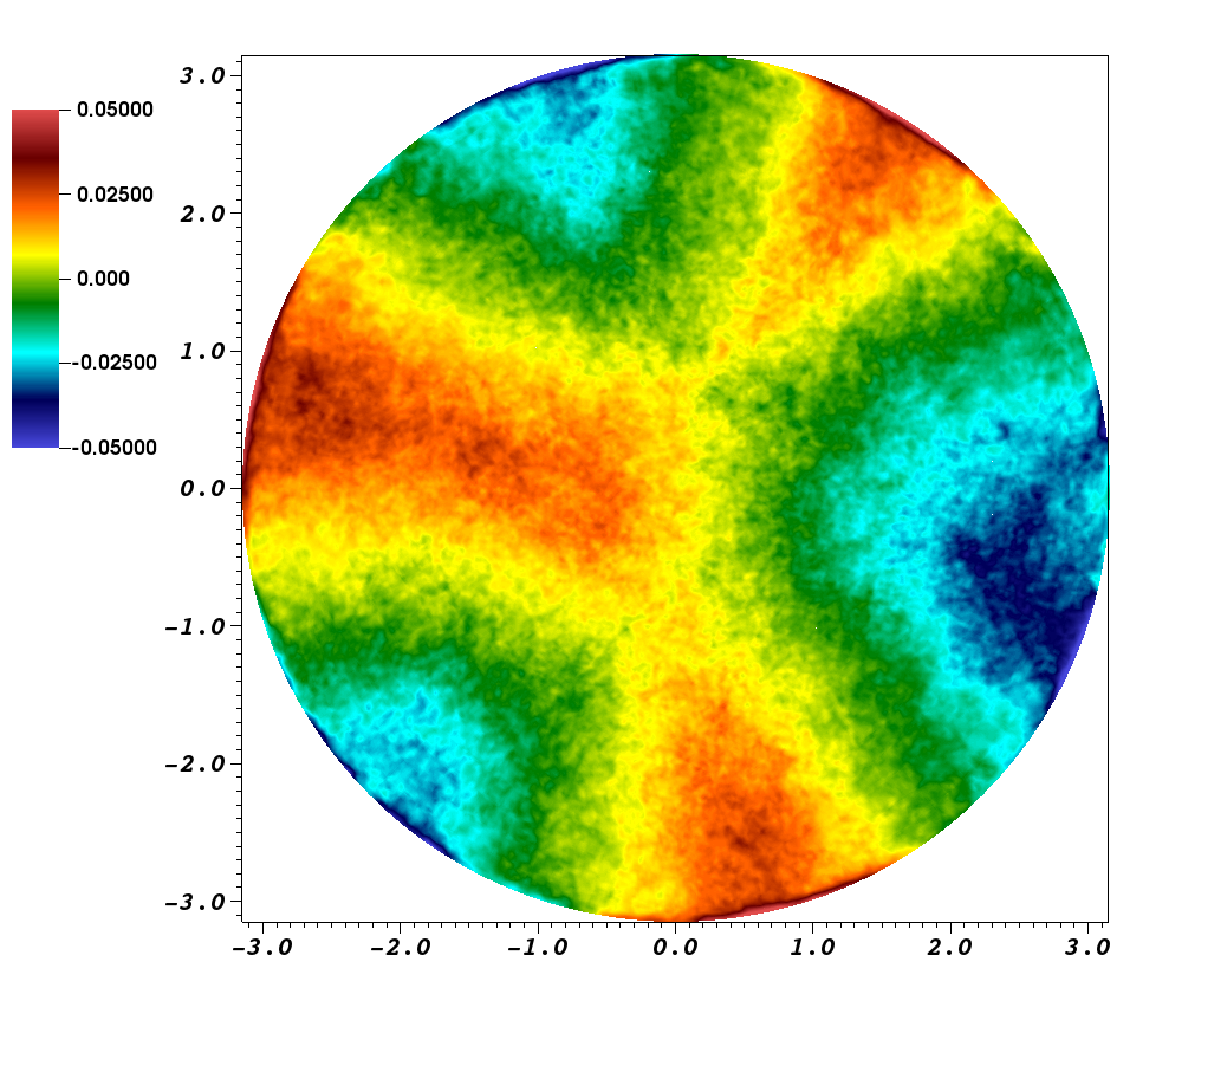
\includegraphics[trim=0cm 2cm 1cm 0cm,clip,width=0.23\textwidth]{TSFP_Filter_Width0002}}{0cm}{-0.1\textwidth}
\topinset{\bfseries(d)}{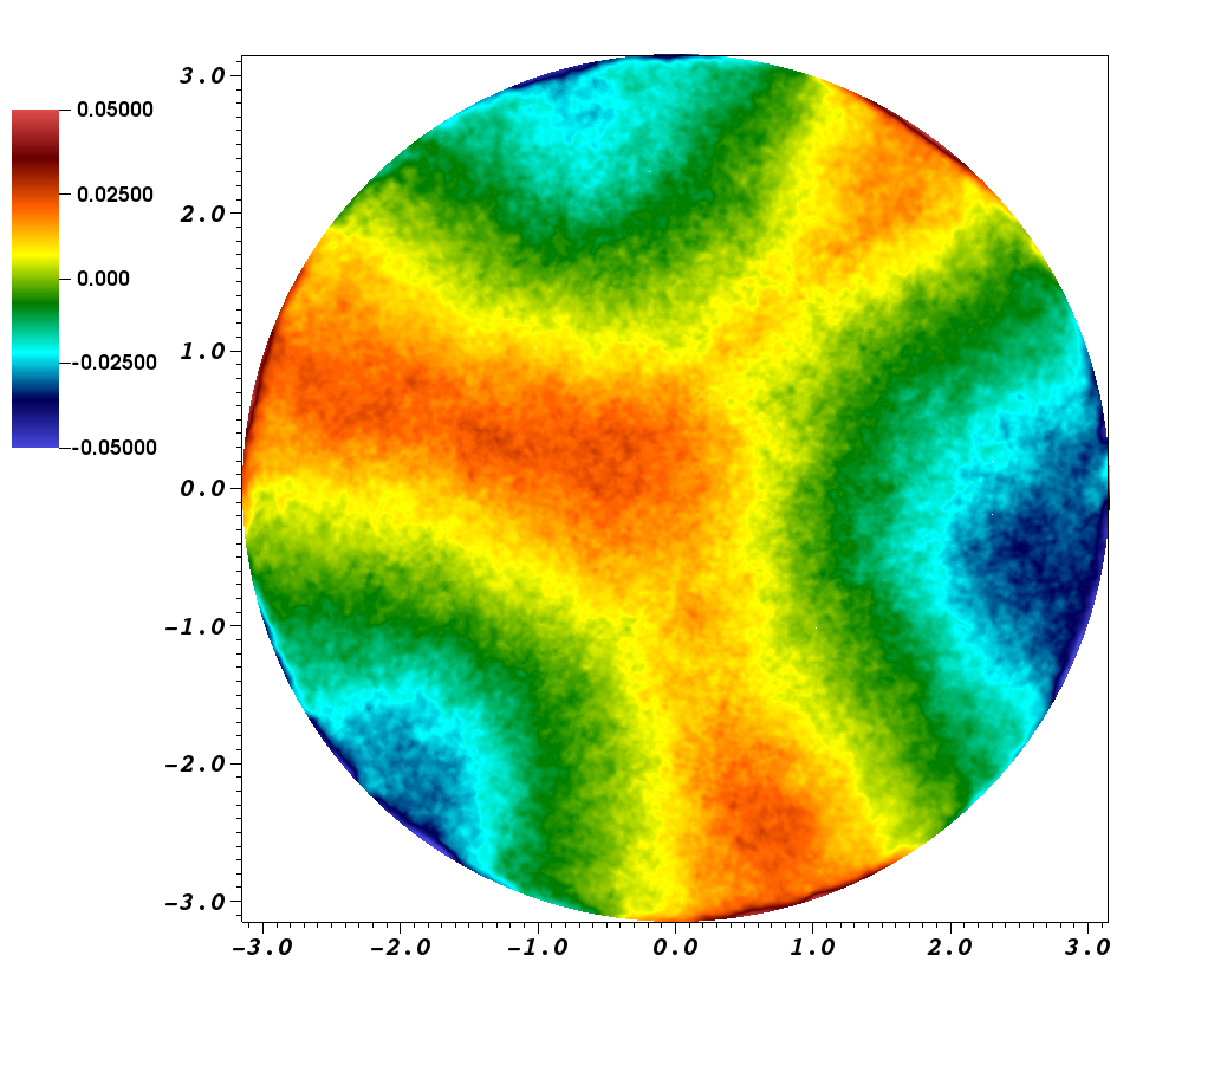
\includegraphics[trim=0cm 2cm 1cm 0cm,clip,width=0.23\textwidth]{TSFP_Filter_Width0003}}{0cm}{-0.1\textwidth}
\caption{Temperature at the mid-plane of the cell plotted with different temporal filtering timescales: instantaneous (a), 1 eddy turnover (b), 10 eddy turnovers (c), 20 eddy turnovers (d).}
\label{fig:filter}
\end{center}
\end{figure*}

In our recent work we studied the large-scale structures in a 6.3 $\Gamma$ RBC cell via direct numerical simulation (DNS) \citep{sakievich2016large}.  This simulation was setup to mirror an experiment conducted by \cite{fernandes2001spatial}. After smoothing out the small-scales with a running time average we observed that the flow organized itself into a hub and spoke like pattern with an updraft in the central region of the cell, and 6 alternating up- and down-drafts near the outer wall.  The hub in this pattern is the central thermal and the spokes are the vortex lines that form between drafts of opposing direction along the outer wall.  A conceptual illustration of the observed pattern's thermal signature is provided in figure~\ref{fig:63ar}. Very similar patterns were seen in the numerical study by \cite{bailon2010aspect}. The large-scale patterns in our recent work \cite{sakievich2016large} and the work of \cite{bailon2010aspect} showed no azimuthal drift or vertical reversal over at least 600 free fall time units ($t_f=\sqrt{h/\beta g \Delta T}$) in numerical simulations. From this we can infer that the large-scale patterns in turbulent RBC are remarkably stable at large $\Gamma$.

\begin{figure}
\centering
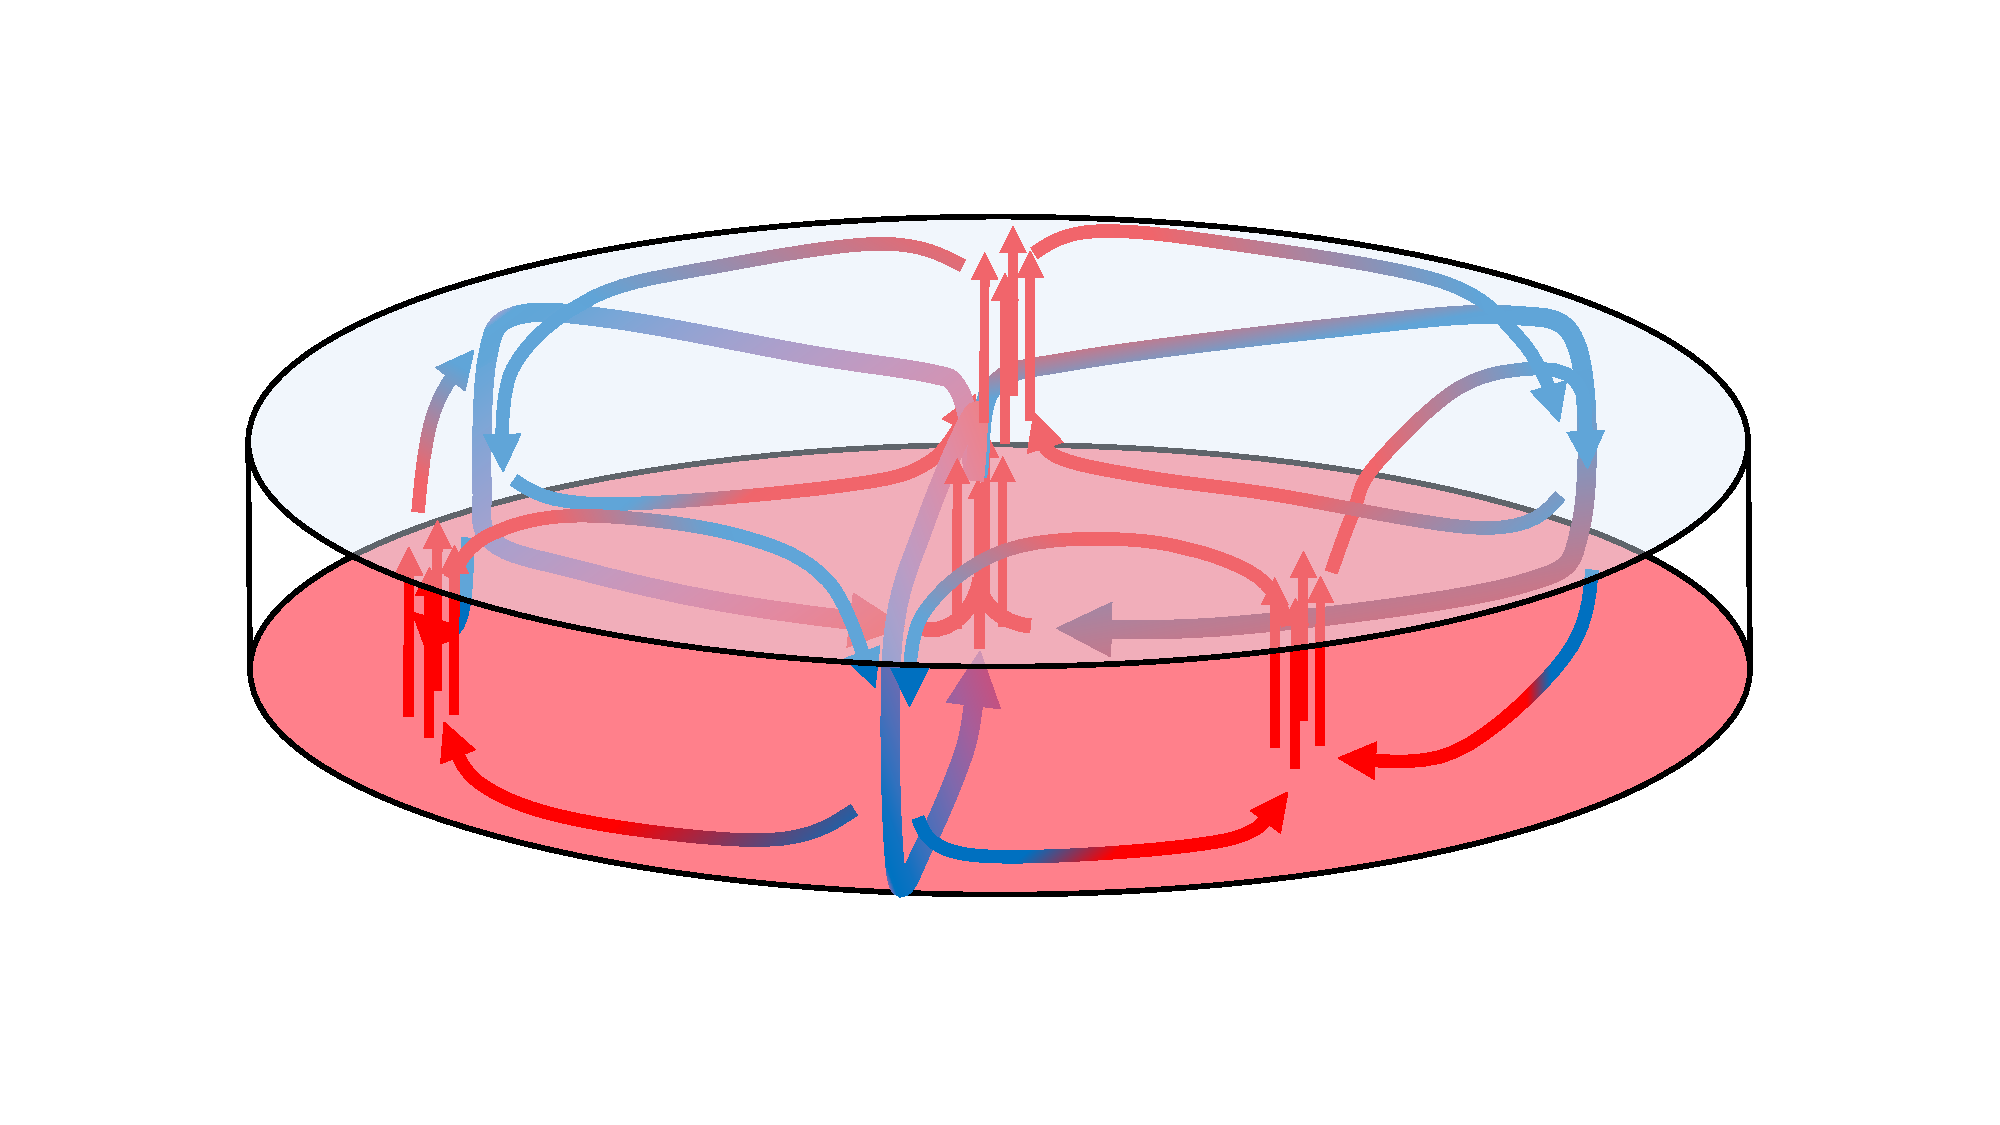
\includegraphics[page=1,trim=4.1cm 3cm 4.1cm 3cm, clip, width=0.3\textwidth]{Ar63Sym}

\caption{Possible patterns at $\Gamma=6.3$.  This pattern is characterized by large-scale updraft in the center, and six large-scale drafts of alternating direction along the cell's side walls. Three dimensional roll-cells are created by connecting each updraft with the neighboring downdrafts. }
\label{fig:63ar}
\end{figure}

\begin{figure}
\begin{center}
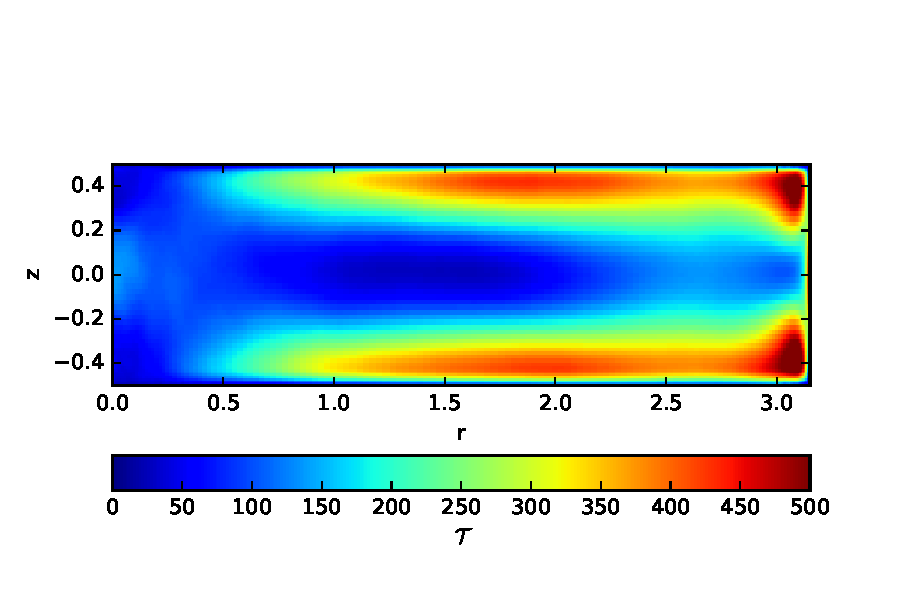
\includegraphics[trim=0cm 1.0cm 0.7cm 2.7cm,clip,width=0.45\textwidth]{IntegralTS_TE}
\caption{Integral timescale for the 6.3 $\Gamma$ simulation with seperation times expressed in freefall time units ($t_f=\sqrt{H/\beta g \Delta T})$}
\label{default}
\end{center}
\end{figure}


We will refer to the observed pattern in figure~\ref{fig:63ar} as $state^+$ because the central column of fluid is an updraft. The persistence of the central column destroys the statistical homogeneity at the center of the cell over the set of realizations in $state^+$. This stands in direct conflict with the idea that as $\Gamma$ is increased the central region of the cell should approach the infinite $\Gamma$ case which is statistically homogeneous over horizontal planes. Clearly, additional states must exist in the infinite ensemble of realizations for this flow, and these states are not represented in this data set even though it was sampled over more than 600$t_f$.  If the temporal sampling were sufficiently extended to truly approach the infinite-time average then an event must occur that will drive the flow into other states.  Possible states should, at the very least, include rotations about the central axis, and a reorganization of the large-scales to where the central region of the cell is characterized by a downdraft.  We will refer to downdraft organization as $state^-$. 


As was mentioned earlier, states that are simply a shift in the pattern's orientation can easily be accounted for by averaging in the homogenous azimuthal direction, as would be sufficient in a low $\Gamma$ case. However, the downdraft pattern in large $\Gamma$ case will require another state of the flow to be sampled. Without this additional state the data set can be considered a conditional average of the infinite time field based on the updraft large-scale organization.  The realizations of the flow in this data set can not be truly statistically independent because the large-scale structures remain highly correlated throughout the time scales achievable in the simulations.

 Traditionally, numerical simulations have relied on temporal averaging for obtaining flow statistics with the expectation that the statistically independent states will be naturally sampled over the duration of the simulation. %While some work has been done to sample multiple states with very long averaging in the low $\Gamma$ case~\cite{brown2005reorientation}, this has not been successful with large aspect ratios. 
 This assumption has two drawbacks: first, as we see in our RBC example, time-scales on which coherent structures evolve can be very significant, so that the amount of run time needed to follow this evolution through many transitions between up- and down-states can be prohibitively large; second, the mechanisms triggering the transitions between the states are still unknown and might not be easily reproducible in continuously executed numerical simulations. For example, carefully conducted experiments in Rayleigh-B\'{e}nard convection involved periodically switching the heat source off and on to produce significant perturbations to trigger statistically independent realizations~\citep{fernandes2001spatial, fernandes2002scaling}.
  
The idea that ensemble averaging, instead or an addition to temporal averaging, is a promising way to improve statistics and models in the simulations has been recognized~\citep{carati1996ensemble, coleman2000numerical}. In these works, initial conditions were selected randomly with the presumption that this initial randomness would yield significantly different realizations. Although intuitively appropriate, this approach might still fail, since the dependence of large-scale structural organization on initial conditions is little understood. It might happen that all initial conditions chosen at random will produce the same state (for example, $state^+$ as in our simulations). A very large number of random realizations might still be biased to one state or another.  
 
In this paper, we propose a simple modification of the conventional sampling and averaging procedures that allows us to select initial conditions for the effective ensemble averaging in a controlled way. With this technique, the additional states that will be sampled are created to possess certain properties (for example, a central downdraft versus updraft) that are missing in the ``base'' realization. By deliberately constructing and sampling specifically manufactured conditions that sample all states, we ensure that the statistics converge to an unbiased estimate of the infinite-time average using a relatively small number of realizations. For example, in this paper we achieve significantly improved statistics with only two realizations, sampling over $state^+$ and $state^-$ as discussed below. This technique can be used to expand the statistical significance of numerical data sets and extend the number of \textit{independent} realizations that can be studied. We will illustrate this technique using our RBC data set, but it can potentially be applied to other flows where there are symmetries that allow solutions in multiple states. 

The main idea behind our technique is to transform an instantaneous realization from the numerical data set into an initial condition for a different state that possesses a desired large-scale structure. For this, we explore symmetries in the inhomogeneous directions. In addition, we require that the transformed data set evolves according to the governing equations. Our central goal for the manipulation performed in this paper is to reverse the flow direction in a central column (updraft versus down-draft) corresponding to $state^+$, identified in figure 2, and its reflection, $state^-$. We recognize that other symmetries (for example, based on the direction of the azimuthal rotation) can also produce other turbulent states.

To reverse the flow direction in the central column, we recast the field so that the structures falling from the cool top plate appear as structures rising from the warm bottom plate and vice versa.  Switching states is performed by transforming the vertical velocity component, vertical coordinate and temperature of a developed turbulent data set at every grid point in the simulation.   The formulas for performing this switch are as follows:
\begin{gather}
z^-(x,y,z^+)=z_{t}+z_{b}-z^+(x,y,z^+)
\label{eq:zmanip} \\
\theta^-(x,y,z^-)=\theta_{t}+\theta_{b}-\theta^+(x,y,z^+)
\label{eq:tmanip}\\
w^-(x,y,z^-)=-w^+(x,y,z^+)
\label{eq:wmanip}
\end{gather}
where the subscripts $t$ and $b$ refer to the values at the top and bottom boundaries, the superscripts $+$ and $-$ refer to the flow states, $z$, $\theta$ and $w$ are the vertical coordinate, dimensionless temperature and vertical velocity, respectively.  The transformation provided by equations~(\ref{eq:zmanip})-(\ref{eq:wmanip}) reflects all variables in the flow about the midplane and preserves the Navier-Stokes equations with the Boussinesq approximation, continuity equation and thermal energy equation exactly. 
%Volume averaged quantities of the transition between $state^+$ and $state^-$ are displayed in figure~\ref{fig:volstat}.  
\begin{figure}
\centering
\topinset{\bfseries{b)}}{\topinset{\bfseries{a)}}{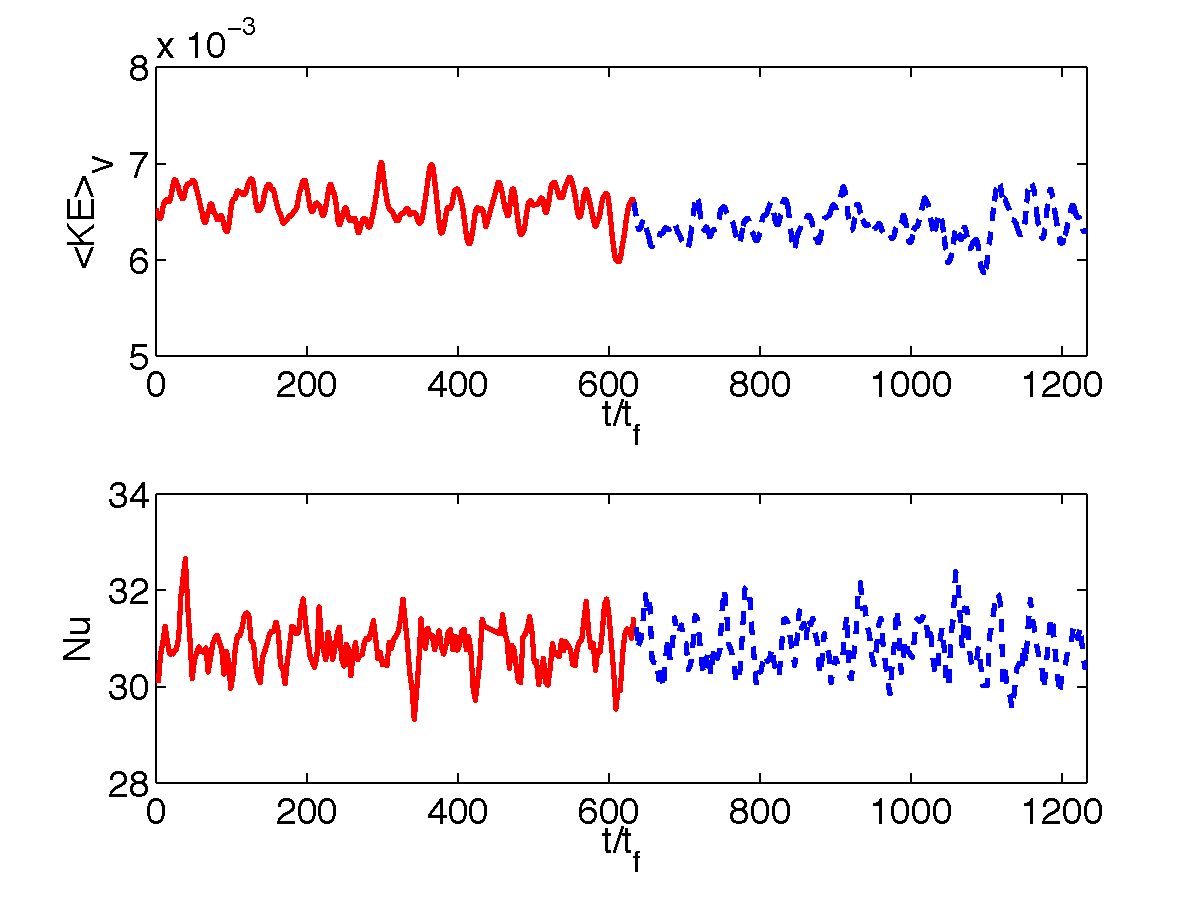
\includegraphics[height=7cm]{VolStats}}{0.25cm}{-4cm}}{3.5cm}{-4cm}
\caption{Temporal evolution of the volume average kinetic energy (a), and Nusselt number (b) are shown in the plots above.  $state^-$ (- -) was initialized from the last time step of $state^+$ (--). }
\label{fig:volstat}
\end{figure}
The plots in figure~\ref{fig:volstat} show identical signatures in the volume averaged kinetic energy and Nusselt number as the transition from $state^+$ to $state^-$ takes place.  These results verify that this methodology preserves the continuity in volume average quantities, such as kinetic energy and total heat flux, during the state transition.
Utilizing this technique to transition between converged states with long term statistical significance has the potential to improve statistical convergence in DNS studies of RBC at a significant reduction in computational expense.  
 
To illustrate this point we have included a comparison with the statistical profiles from experiments of \cite{fernandes2001spatial} and our previous work \citep{sakievich2016large} in figure~\ref{fig:profs}. These profiles have been normalized by Deardorff's velocity scale $w*=(\beta g Q_o h)^{1/3}$~\citep{deardorff1970convective} where $Q_o$ is the kinematic heat flux.
\begin{figure}
\centering
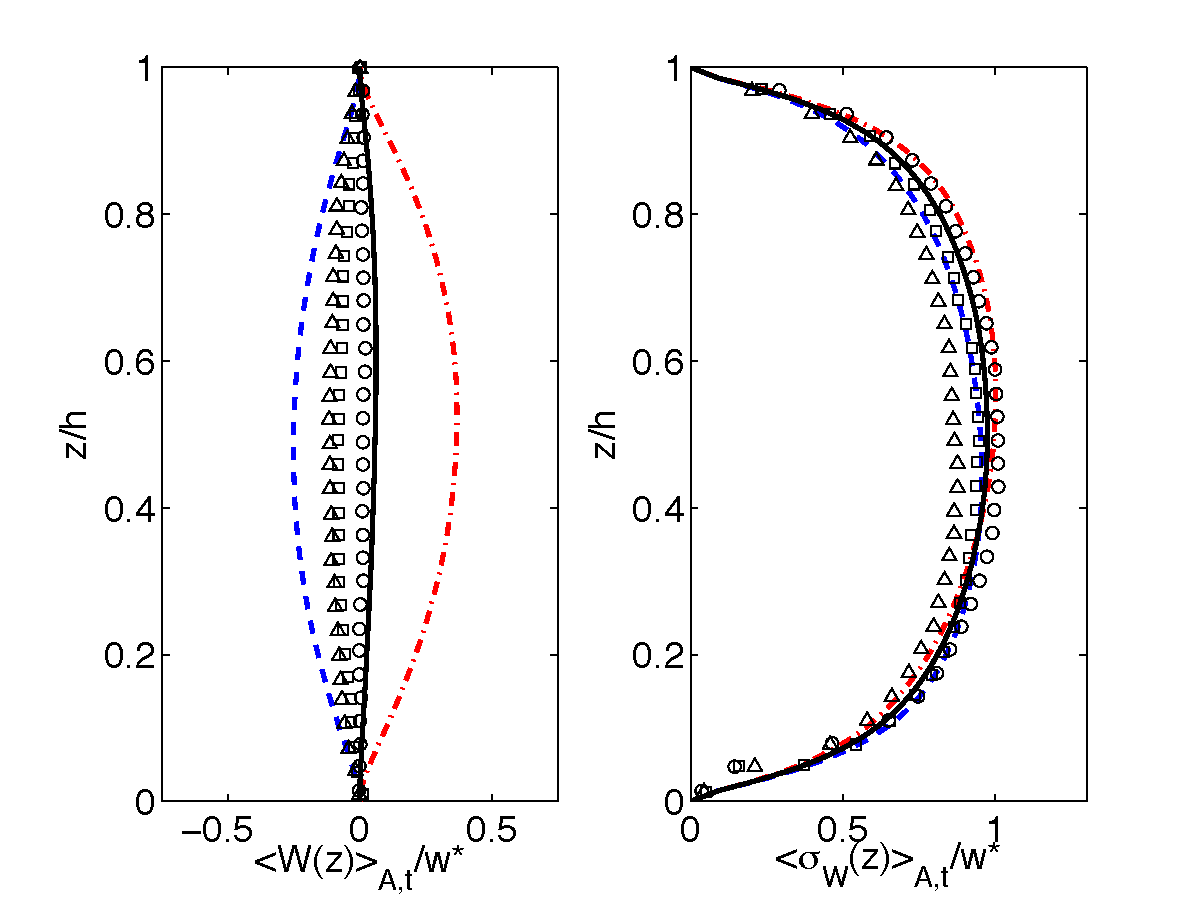
\includegraphics[height=6cm]{PRL_Fig1}
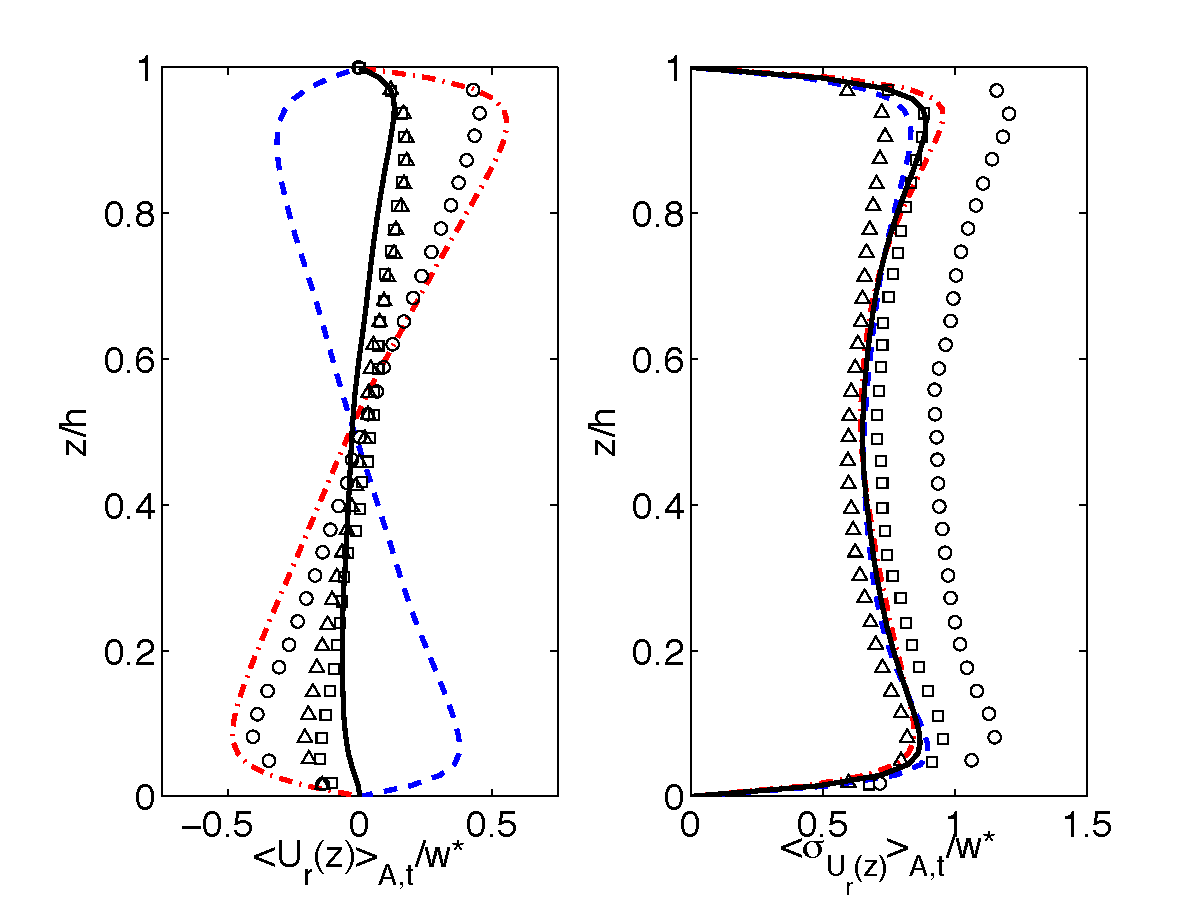
\includegraphics[height=6cm]{PRL_Fig2}
\caption{Ensemble and horizontally averaged mean (left) and r.m.s. (right) vertical (top) and radial (bottom) velocity profiles normalized by Deardorff's velocity scale $w*$: DNS: $Ra=9.6\times10^7$, averaging domain $\Omega_F$ where red ($- \cdot$ ) is $state^+$, blue (- -) is $state^-$ and black (--) is the average of $state^+$ and $state^-$; Experiment: $Ra=6\times10^7$ ($\medtriangleup$), $Ra=2\times10^8$ ($\medsquare$),  $Ra=1\times10^9$ ($\medcircle$)}
\label{fig:profs}
\end{figure}

The profiles generated in figure~\ref{fig:profs} are taken from within the core region of the 6.3 $\Gamma$ RBC cell with a radius of $0.925h$. It should be noted that the experimental mean vertical velocity profiles decrease in magnitude and the r.m.s vertical velocity profile's magnitude increases with $Ra$.  Since the forcing within the cell increases with $Ra$ the characteristic instantaneous velocity increases as the vertical r.m.s profile indicates. We hypothesize that the reason for the decay of the mean velocity in the experimental profiles is that the antisymmetric states were more evenly accounted for in Fernandes ensemble averages with higher $Ra$~\citep{fernandes2001spatial}. When the original DNS results ($state^+$ only) are compared against the experiment we see that the r.m.s profiles fall within $\sim11$\% in a pointwise comparison and that the mean profiles are dramatically over predicted.  However, when the $state^+$ and $state^-$ are averaged together, the mean velocity profiles are very close to the expected (zero) value of the infinite-time average and the r.m.s profiles show an excellent match with the experimental results. This is truly remarkable when one considers that each instance of Fernades' ensemble average (with the  total of 300 instances) was also temporally averaged over a greater time period than our entire simulation. By our estimates it would take us $O(10^8)$ CPU hours to recreate Fernandes experiment on our current grid (and the ability to recreate the desired uncorrelated large-scale patterns with just random initializations still could not be guaranteed). However, the results presented in this paper took $O(10^5)$ CPU hours to produce.  Perhaps the most exciting observation is that the profiles in figure~\ref{fig:profs} clearly show that we were able to obtain a net downdraft in the central region of the cell over the sampling time of our second state.   This shows that we were able to perform a targeted manipulation of instantaneous data to trigger a new state of the large-scale structures. 



\section*{SUMMARY AND CONCLUSIONS}

In summary we have discussed the challenges in obtaining the flow statistics that would converge to an infinite-time average in numerical simulations of turbulent flows and the bias that can be introduced due to insufficient sampling of flow states.
% dictated by inhomogeneous directions. 
Failure to recognize insufficient sampling can lead to variance in the statistics of stationary processes which are due to the correlation of slowly evolving large-scale structures that can persist well beyond the standard integral time scales.  We used our recent numerical simulation of a 6.3 $\Gamma$ RBC cell to provide an example of how this can occur.  The results from this simulation were obtained with a high-order method and were numerically well resolved, as well as yielded longer than average temporal sampling~\cite{sakievich2016large}, but the central region of the cylinder showed inhomogeneous nature due to a large-scale updraft persisting in the cell's core.  The only way to resolve this issue is to average these results with another state of the flow field with a downdraft in the center.  We then presented a methodology for triggering this state using the inherent symmetries in the inhomogeneous vertical direction that didn't alter the net kinetic or thermal energy in the fully developed turbulent field. The application of this methodology showed that a net downdraft was indeed created in the region of interest and that this downdraft remained dominant over at least the same temporal averaging period that was used to collect the first flow state. 
This method has the potential for application to other flows that have multiple, long-lived states and an exploitable symmetry. 
%Since the transformation used in this methodology is based on the general principle of symmetry it has excellent potential to be applied to additional turbulent flows beyond RBC. 

\section{ACKNOWLEDGMENTS}
We would like to acknowledge U.S. National Science Foundation Grants CBET-1335731 and CMMI-1250124, XSEDE allocation TG-ENG140002, and the Arizona State University (2013/2016-MAE- 105) Dean's Fellowship for supporting this work. 
%%%%%%%%%%%%%%%%%%%%%%%%%%%%%%%%%%%%%%%%%%%%%%%%%%%%%%%%%%%%%%%%%%%%%%%
\bibliographystyle{tsfp}
\bibliography{supercoherent}
% In this example, BibTeX is used
% For users not familiar with LaTeX, the bibliography can be typed in directly. In this case, comment the two lines above.
%%%%%%%%%%%%%%%%%%%%%%%%%%%%%%%%%%%%%%%%%%%%%%%%%%%%%%%%%%%%%%%%%%%%%%%
%\section*{SAMPLE REFERENCES}
%
%Kwon, O. K., and Pletcher, R. H., 1981, "Prediction of the Incompressible Flow Over a Rearward-Facing Step", Technical Report HTL-26, CFD-4, Iowa State Univ., Ames, IA.
%
%Lee, Y., Korpela, S. A., and Horne, R. N., 1982, "Structure of Multi-Cellular Natural Convection in a Tall Vertical Annulus," Proceedings, 7th International Heat Transfer Conference, U. Grigul et al., ed., Hemisphere Publishing Corp., Washington, D.C., Vol. 2, pp. 221-226.
%
%Sparrow, E. M., 1980a, "Fluid-to-Fluid Conjugate Heat Transfer for a Vertical Pipe - Internal Forced Convection and External Natural Convection", ASME Journal of Heat Transfer, Vol. 102, pp. 402-407.
%
%Sparrow, E. M., 1980b, "Forced-Convection Heat Transfer in a Duct Having Spanwise-Periodic Rectangular Protuberances", Numerical Heat Transfer, Vol. 3, pp. 149- 167.
%
%Tung, C. Y., 1982, Evaporative Heat Transfer in the Contact Line of a Mixture, Ph.D. Thesis, Rensselaer Polytechnic Institute, Troy, NY.

%%%%%%%%%%%%%%%%%%%%%%%%%%%%%%%%%%%%%%%%%%%%%%%%%%%%%%%%%%%%%%%%%%%%%%


\end{document}
